% Flight Test Card Start

% =============================================================================#
% created by Kevin Horton, 2011
% 
% This file is part of ft_program.
% 
%     ft_program is free software: The exectuable files are licensed under the
%     Gnu Public License, but the latex files, including this file, are placed 
%     in the public domain.  
% 
% =============================================================================#

% NOTES
% need to use \noindent at the start of each new para to avoid an indent.
% Has several placeholders, to be searched and replaced by a perl script:
% <<<Flt_No>>>
% <<<Date>>>
%<<<Pilot>>>
%<<<FTE>>>
%<<<Purpose>>>


%\documentclass[letterpaper,10pt,halfparskip]{scrartcl}
%\documentclass[10pt,halfparskip]{scrartcl}
% \documentclass[12pt,halfparskip]{scrartcl}
\documentclass[14pt,halfparskip]{scrartcl}
%\documentclass{article}
\usepackage[OT1]{fontenc}
\usepackage[latin1]{inputenc}
\usepackage{boxedminipage}
\usepackage{calc} % used by the geometry package to do calculations
\usepackage{color}
\usepackage{extsizes} % for extra font sizes
\usepackage{geometry}
%  \geometry{verbose,letterpaper,tmargin=0.25 in,left=1 in,right=0.25 in,bmargin=0.75 in}
%  \geometry{verbose,paperwidth=5.5 in,paperheight=8.5in,hoffset=-0.25 in,tmargin=0.75 in,left=1 in,right=0 in,bmargin=0.5 in,footskip=20 pt}
 % 0.25 in right margin needed if making 2 pages per page in the pdf file.
  \geometry{reset,verbose,a4paper,tmargin=1 in,left=0.25 in,right=0.25 in,bmargin=0.5 in,footskip=20 pt}
  % 0.15 in right margin needed if doing one page per page, and using Preview to make 2 pages per page.
%  \geometry{reset,verbose,a4paper,tmargin=0.5 in,left=1 in,right=0.15 in,bmargin=0.5 in,footskip=20 pt}
\usepackage{graphicx}
\usepackage{layouts}
\usepackage{multirow}
\usepackage{paralist} % to get compact list environments
\usepackage{pifont} % to get dingbats
\usepackage{ragged2e} % to get the justifying option to make NOTES
\usepackage{tabularx}
\usepackage{textcomp} % for to get degree symbols from \textdegree
%\usepackage[cross,letter]{crop}

% following lengths are used to set row widths to fit the text
\newlength{\colOne}
\newlength{\colTwo}
\newlength{\colThree}
\newlength{\colFour}
\newlength{\colFive}
\newlength{\colSix}
\newlength{\colSeven}
\newlength{\colEight}

% Define Test Point environment
% Concept from TLC2 page 849.
\newcounter{TP} \newsavebox{\TestPointName}
\newenvironment{TestPoint}[1]
   {\stepcounter{TP}
    \noindent\begin{minipage}{\linewidth}
      \Large{\textsf{\textbf{\arabic{TP}. #1}}}\hfill\normalfont\normalsize \begin{boxedminipage}{0.75 in}\textcolor{white}{g}\end{boxedminipage}
%      \Large{\textsf{\textbf{\arabic{TP}. #1}}}\hfill\normalfont\normalsize Start \begin{boxedminipage}{0.75 in}\textcolor{white}{g}\end{boxedminipage}
      \vspace{0.15 in}\par}
   {\par\hfill Complete \begin{boxedminipage}{0.75 in}\textcolor{white}{g}\end{boxedminipage}
   \noindent\rule{\linewidth}{1mm}\vspace{0.15 in}
    \end{minipage}}

%% New environment for NOTES, CAUTIONS and WARNINGS
\newcounter{oldparindent}
\newenvironment{Note}[1][NOTE]
  {
    \setcounter{oldparindent}{\parindent} 
    \begin{quote}
    \centering{\textbf{#1}}
    \\ 
    \justifying  
    \parindent=0pt
  }
  {
    \parindent \value{oldparindent}pt
    \end{quote}
  }

%% New environment for NOTES, CAUTIONS and WARNINGS in checklists
%% Same as normal notes, but no indent.
\newenvironment{Note2}[1][NOTE]
  {
    \setcounter{oldparindent}{\parindent} 
    \centering{\textbf{#1}}
    \\ 
    \justifying  
    \parindent=0pt
  }
  {
    \parindent \value{oldparindent}pt
  }

% used for approach to stall, and other places
\newcounter{TrimSpeed}


% adjust paragraph separation for compactenum environment
%\setlength\plitemsep{2 pt}

\begin{document}

%% Following three lines show a minipage diagram, with margins shown.  Seems to need layouts package.
%\currentpage
%\setlayoutscale{0.5}
%\pagedesign

%\noindent\begin{tabularx}{\linewidth - 10 pt}{llXrlXrl}
\noindent\begin{tabularx}{\linewidth - 10 pt}{llXrlXrl}
  <<<type>>>&<<<aircraft>>>&&Flt \#:&<<<flt_no>>>&&Date:&<<<date>>>
  \end{tabularx}
  
\noindent\begin{tabularx}{\linewidth - 10 pt}{llX|l|c|c|}
  \cline{4-6}
  &&&&Time&Fuel\\
  &&&&&(USG)\\
  \cline{4-6}
  Weight:&<<<to_wt>>> lb.&&Start&&\\
  \cline{4-6}
  CG:&<<<to_cg>>>" aft of datum&&Taxi&&\\
  \cline{4-6}
  &&&Take-off&&\\
  \cline{4-6}
  Pilot:&<<<pilot>>>&&Landing&&\\
  \cline{4-6}
  FTE:&<<<fte>>>&&Stop&&\\
  \cline{4-6}
  &&&Shut Down&&\\
  \cline{4-6}
  \end{tabularx}

%PURPOSE
%\noindent\rule{\linewidth}{1mm}\vspace{0.2 in}
\noindent\rule{\linewidth}{1mm}
%\noindent\rule{\linewidth}{1mm}\vspace{0.1 in}
 \section*{PURPOSE}
    <<<purpose>>>
  
% WEATHER
%\noindent\rule{\linewidth}{1mm}\vspace{0.2 in}
\noindent\rule{\linewidth}{1mm}
%\noindent\rule{\linewidth}{1mm}\vspace{0.1 in}
\section*{WEATHER}
% set widths for table
\settowidth\colOne{LAND}
\settowidth\colTwo{ATIS}
\settowidth\colThree{Wind}
\settowidth\colFour{Vis}
\settowidth\colSix{Temp}
\settowidth\colSeven{Alt.}
\noindent\begin{tabularx}{\linewidth - 10 pt}{|p{\colOne}|p{\colTwo}|p{\colThree}|p{\colFour}|X|p{\colSix}|p{\colSeven}|}
  \hline
  &ATIS&Wind&Vis&Weather&Temp.&Alt.\\
  \hline
  \hline
  T/O&&&&&&\\
  \hline
  LAND&&&&&&\\
  \hline
  \end{tabularx}
  
%LIMITATIONS
\noindent\rule{\linewidth}{1mm}\vspace{0.1 in}
%\noindent\rule{\linewidth}{1mm}
\noindent\begin{minipage}{\linewidth}
\section*{LIMITATIONS}
<<<limitations>>>
\end{minipage}

\noindent\begin{minipage}{\linewidth}
  \section*{WEIGHT AND BALANCE}
    \begin{center}
    \begin{tabular}{|l|r|r|r|}
      \hline
      \multicolumn{1}{|c|}{ITEM}&\multicolumn{1}{c|}{WEIGHT}&\multicolumn{1}{c|}{ARM}&\multicolumn{1}{c|}{MOMENT}\\
      &\multicolumn{1}{c|}{(lb)}&\multicolumn{1}{c|}{(in.)}&\multicolumn{1}{c|}{(lb-in.)}\\
      \hline
      \hline
      Empty Weight&<<<empty_wt>>>&<<<empty_arm>>>&<<<empty_moment>>>\\
      \hline
      Pilot&<<<pilot_wt>>>&<<<pilot_arm>>>&<<<pilot_moment>>>\\
      \hline
      Rear Seat&<<<rear_seat_wt>>>&<<<rear_seat_arm>>>&<<<rear_seat_moment>>>\\
      \hline
      Forward Baggage&<<<fwd_baggage_wt>>>&<<<fwd_baggage_arm>>>&<<<fwd_baggage_moment>>>\\
      \hline
      Rear Baggage&<<<rear_baggage_wt>>>&<<<rear_baggage_arm>>>&<<<rear_baggage_moment>>>\\
      \hline
      Rear Baggage Shelf&<<<rear_baggage_shelf_wt>>>&<<<rear_baggage_shelf_arm>>>&<<<rear_baggage_shelf_moment>>>\\
      \hline
      Ballast 1&<<<ballast1_wt>>>&<<<ballast1_arm>>>&<<<ballast1_moment>>>\\
      \hline
      Ballast 2&<<<ballast2_wt>>>&<<<ballast2_arm>>>&<<<ballast2_moment>>>\\
      \hline
      \hline
      \textbf{Zero Fuel Weight}&\textbf{<<<zfw>>>}&\textbf{<<<zfw_cg>>>}&<<<zfw_moment>>>\\
      \hline
      \hline
      Fuel&<<<fuel_wt>>>&<<<fuel_arm>>>&<<<fuel_moment>>>\\
      \hline
      \hline
      \textbf{Weight at Engine Start}&\textbf{<<<to_wt>>>}&\textbf{<<<to_cg>>>}&<<<to_moment>>>\\
      \hline
      \end{tabular}

%% =============================================================================#
% created by Kevin Horton, 2011
% 
% This file is part of ft_program.
% 
%     ft_program is free software: The exectuable files are licensed under the
%     Gnu Public License, but the latex files, including this file, are placed 
%     in the public domain.  
%
% =============================================================================#
% GNUPLOT: LaTeX picture with Postscript
\begingroup
  \makeatletter
  \providecommand\color[2][]{%
    \GenericError{(gnuplot) \space\space\space\@spaces}{%
      Package color not loaded in conjunction with
      terminal option `colourtext'%
    }{See the gnuplot documentation for explanation.%
    }{Either use 'blacktext' in gnuplot or load the package
      color.sty in LaTeX.}%
    \renewcommand\color[2][]{}%
  }%
  \providecommand\includegraphics[2][]{%
    \GenericError{(gnuplot) \space\space\space\@spaces}{%
      Package graphicx or graphics not loaded%
    }{See the gnuplot documentation for explanation.%
    }{The gnuplot epslatex terminal needs graphicx.sty or graphics.sty.}%
    \renewcommand\includegraphics[2][]{}%
  }%
  \providecommand\rotatebox[2]{#2}%
  \@ifundefined{ifGPcolor}{%
    \newif\ifGPcolor
    \GPcolorfalse
  }{}%
  \@ifundefined{ifGPblacktext}{%
    \newif\ifGPblacktext
    \GPblacktexttrue
  }{}%
  % define a \g@addto@macro without @ in the name:
  \let\gplgaddtomacro\g@addto@macro
  % define empty templates for all commands taking text:
  \gdef\gplbacktext{}%
  \gdef\gplfronttext{}%
  \makeatother
  \ifGPblacktext
    % no textcolor at all
    \def\colorrgb#1{}%
    \def\colorgray#1{}%
  \else
    % gray or color?
    \ifGPcolor
      \def\colorrgb#1{\color[rgb]{#1}}%
      \def\colorgray#1{\color[gray]{#1}}%
      \expandafter\def\csname LTw\endcsname{\color{white}}%
      \expandafter\def\csname LTb\endcsname{\color{black}}%
      \expandafter\def\csname LTa\endcsname{\color{black}}%
      \expandafter\def\csname LT0\endcsname{\color[rgb]{1,0,0}}%
      \expandafter\def\csname LT1\endcsname{\color[rgb]{0,1,0}}%
      \expandafter\def\csname LT2\endcsname{\color[rgb]{0,0,1}}%
      \expandafter\def\csname LT3\endcsname{\color[rgb]{1,0,1}}%
      \expandafter\def\csname LT4\endcsname{\color[rgb]{0,1,1}}%
      \expandafter\def\csname LT5\endcsname{\color[rgb]{1,1,0}}%
      \expandafter\def\csname LT6\endcsname{\color[rgb]{0,0,0}}%
      \expandafter\def\csname LT7\endcsname{\color[rgb]{1,0.3,0}}%
      \expandafter\def\csname LT8\endcsname{\color[rgb]{0.5,0.5,0.5}}%
    \else
      % gray
      \def\colorrgb#1{\color{black}}%
      \def\colorgray#1{\color[gray]{#1}}%
      \expandafter\def\csname LTw\endcsname{\color{white}}%
      \expandafter\def\csname LTb\endcsname{\color{black}}%
      \expandafter\def\csname LTa\endcsname{\color{black}}%
      \expandafter\def\csname LT0\endcsname{\color{black}}%
      \expandafter\def\csname LT1\endcsname{\color{black}}%
      \expandafter\def\csname LT2\endcsname{\color{black}}%
      \expandafter\def\csname LT3\endcsname{\color{black}}%
      \expandafter\def\csname LT4\endcsname{\color{black}}%
      \expandafter\def\csname LT5\endcsname{\color{black}}%
      \expandafter\def\csname LT6\endcsname{\color{black}}%
      \expandafter\def\csname LT7\endcsname{\color{black}}%
      \expandafter\def\csname LT8\endcsname{\color{black}}%
    \fi
  \fi
  \setlength{\unitlength}{0.0500bp}%
  \begin{picture}(5760.00,5040.00)%
    \gplgaddtomacro\gplbacktext{%
      \csname LTb\endcsname%
      \put(1210,704){\makebox(0,0)[r]{\strut{} 1100}}%
      \put(1210,1156){\makebox(0,0)[r]{\strut{} 1200}}%
      \put(1210,1609){\makebox(0,0)[r]{\strut{} 1300}}%
      \put(1210,2061){\makebox(0,0)[r]{\strut{} 1400}}%
      \put(1210,2513){\makebox(0,0)[r]{\strut{} 1500}}%
      \put(1210,2966){\makebox(0,0)[r]{\strut{} 1600}}%
      \put(1210,3418){\makebox(0,0)[r]{\strut{} 1700}}%
      \put(1210,3870){\makebox(0,0)[r]{\strut{} 1800}}%
      \put(1210,4323){\makebox(0,0)[r]{\strut{} 1900}}%
      \put(1210,4775){\makebox(0,0)[r]{\strut{} 2000}}%
      \put(1342,484){\makebox(0,0){\strut{} 78}}%
      \put(1751,484){\makebox(0,0){\strut{} 79}}%
      \put(2159,484){\makebox(0,0){\strut{} 80}}%
      \put(2568,484){\makebox(0,0){\strut{} 81}}%
      \put(2977,484){\makebox(0,0){\strut{} 82}}%
      \put(3386,484){\makebox(0,0){\strut{} 83}}%
      \put(3794,484){\makebox(0,0){\strut{} 84}}%
      \put(4203,484){\makebox(0,0){\strut{} 85}}%
      \put(4612,484){\makebox(0,0){\strut{} 86}}%
      \put(5020,484){\makebox(0,0){\strut{} 87}}%
      \put(5429,484){\makebox(0,0){\strut{} 88}}%
      \put(308,2739){\rotatebox{-270}{\makebox(0,0){\strut{}Weight (lb)}}}%
      \put(3385,154){\makebox(0,0){\strut{}CG (inches aft of datum)}}%
      \put(1751,3735){\makebox(0,0)[l]{\strut{}\ding{172}}}%
      \put(1751,2604){\makebox(0,0)[l]{\strut{}\ding{173}}}%
      \put(4714,3735){\makebox(0,0)[l]{\strut{}\ding{174}}}%
      \put(1342,-651){\makebox(0,0)[l]{\strut{}\ding{172} Restricted Aerobatic Weight/CG Envelope}}%
      \put(1342,-968){\makebox(0,0)[l]{\strut{}\ding{173} Aerobatic Weight/CG Envelope}}%
      \put(1342,-1284){\makebox(0,0)[l]{\strut{}\ding{174} Normal Weight/CG Envelope}}%
    }%
    \gplgaddtomacro\gplfronttext{%
      \put(4442,4602){\makebox(0,0)[r]{\strut{}Fuel Burn}}%
      \put(2328,3214){\makebox(0,0)[l]{\strut{}Start}}%
      \put(2351,2047){\makebox(0,0)[l]{\strut{}Zero Fuel}}%
    }%
    \gplbacktext
    \put(0,0){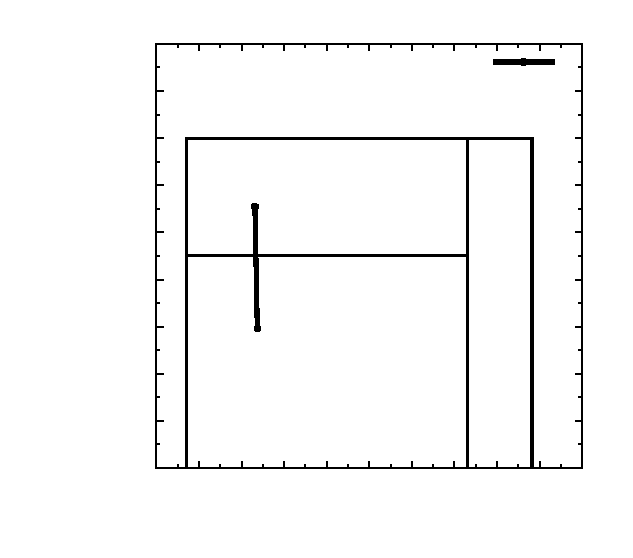
\includegraphics{/Users/kwh/sw_projects/hg/ft_program/wb/wb_chart}}%
    \gplfronttext
  \end{picture}%
\endgroup

\input{<<<wb_chart>>>}
\end{center}
\end{minipage}

\clearpage
\begin{TestPoint}{BEFORE START}
  \begin{tabular}{p{6cm}|p{2cm}|l}
    \multicolumn{3}{l}{\textbf{** SET ANALOG ALTIMETER **}}\\
    \multicolumn{3}{l}{\textbf{** SET EFIS ALTIMETER TO 29.92 **}}\\
    \multicolumn{3}{l}{\textbf{** START DATA RECORDING **}}\\
  
    \cline{2-2}
    Oil Temp&&\\
    \cline{2-2}
    \multicolumn{3}{l}{Check all engine parametres OK.}
    \end{tabular}
  \end{TestPoint}

\begin{TestPoint}{ENGINE START}
  \begin{tabular}{p{6cm}|p{2cm}|}
    \cline{2-2}
%    Time&\\
%    \cline{2-2}
    Fuel&\\
    \cline{2-2}
    EIS OK after start?&\\
    \cline{2-2}
    Taxi Time&\\
    \cline{2-2}
    Taxi Fuel&\\
    \cline{2-2}
    \end{tabular}
  \vspace{0.1 in}\\
  % =============================================================================#
% created by Kevin Horton, 2011
% 
% This file is part of ft_program.
% 
%     ft_program is free software: The exectuable files are licensed under the
%     Gnu Public License, but the latex files, including this file, are placed 
%     in the public domain.  
%
% =============================================================================#

 \subsubsection*{Observations}
  \begin{tabularx}{\linewidth}{X}
    \hline
    \\
    \hline
    \\
    \hline
    \\
    \hline
    \end{tabularx}

  \end{TestPoint}
  
\begin{TestPoint}{RUN UP}
  % =============================================================================#
% created by Kevin Horton, 2011
% 
% This file is part of ft_program.
% 
%     ft_program is free software: The exectuable files are licensed under the
%     Gnu Public License, but the latex files, including this file, are placed 
%     in the public domain.  
%
% =============================================================================#

 \subsubsection*{Observations}
  \begin{tabularx}{\linewidth}{X}
    \hline
    \\
    \hline
    \\
    \hline
    \\
    \hline
    \end{tabularx}

  \end{TestPoint}
